\chapter*{課程學習反思}
Neural Network 的學習,主要是透過微分。與課程之前,我已預先習得了相關內容,如指數、對數的微分以及最重要的 chain rule 。運用一些統計學的技巧也可以使訓練加快。

人類在處理數據資料(如房價相關變數)時,會進行加權或是更複雜的動作。加權可以表示此變數的影響程度,權值大小則是由人類決定(根據經驗),進而分析預測出結果(如房價)。在統計學上,迴歸分析是用於討論自變數與應變數的關係(如房價相關變數與房價),取得適當的權值以進行預測。在 Neural Network 之前,人類常會用此種方法去預測。 Neural Network 的學習很可能就是從這裡發展的(透過微分的學習)。下圖為運用 Tensorflow 計算迴歸線的結果,可以看到預測(藍線)已經十分貼合實際的數據(紅點)。

\begin{figure}[H]
    \centering
    \caption{用 Tensorflow 計算迴歸線}
    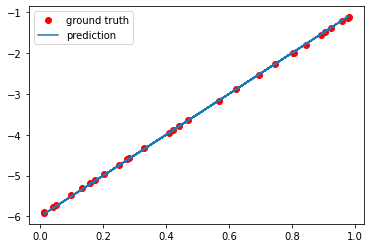
\includegraphics[width=.7\columnwidth]{linear_regression}
\end{figure}



Neural Network 之所以強大, 就是因為「深度」。他可分析出的特徵比以前的方法都還強大,更重要的是還能「學習」。只要提供資料,他就可以自行去找出資料中的特徵。

在課程之餘,我也參加了 Kaggle Digit Recognizer 競賽,實際動手總是比純聽課還要有更好的效果。在比賽中,我原本 Neural Network 所設置的層數較多,後來經過了一些調整,發現2層卷積層接上2層全連結層配上一些 Dropout 層效果最佳,最終達到超過99\%的 accuracy 。

\begin{figure}[H]
    \centering
    \caption{Kaggle 競賽排名}
    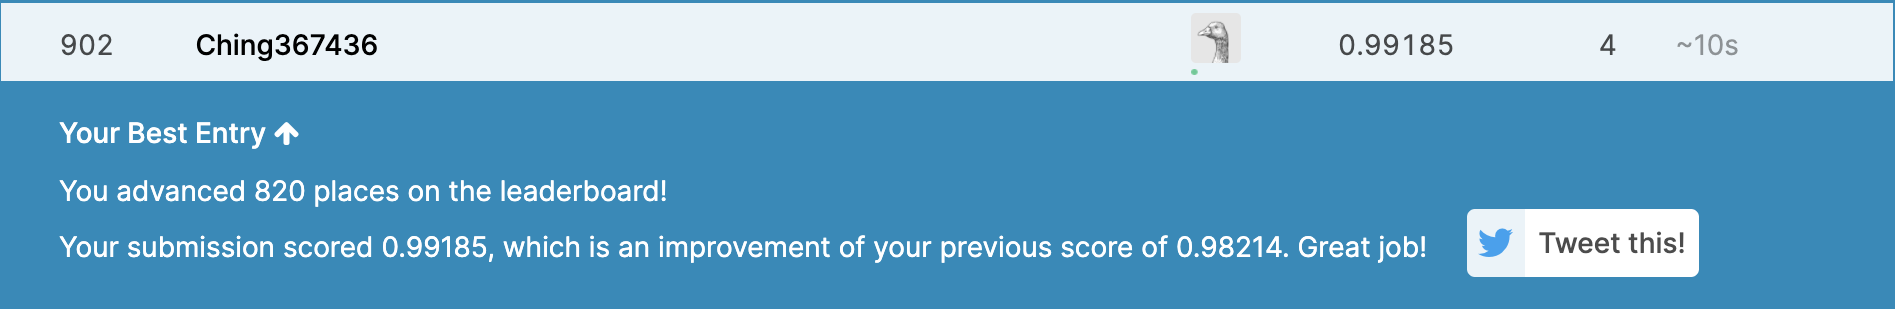
\includegraphics[width=.7\columnwidth]{kaggle_rank}
\end{figure}


在課程之中,我完成了音樂生成 、 Neural Style Transfer 、 Object Detection 等現今常見的 Neural Network 應用。其中,Neural Style Transfer 是我最感興趣的部分,竟然可以從已訓練好的 Neural Network 中這樣子取得 $ Style $,這讓我十分的佩服。算式如下,簡單來講就是一張圖片出現某種特徵時,是否伴隨這另一種特徵,如紅底伴隨著斜線出現、漩渦伴隨著藍與黃色等。這些特徵通常都出現在 Neural Network 的中間層,所以通常採用中間層的輸出。

\[
    G_{gram} = A_{unrolled} A^{T}_{unrolled}
\]

\begin{center}
    $ A $ 表示 Convolutional Neural Network (中間層)的輸出

    $ G_{gram} $ 則是 gram matrix 
\end{center}

在這個課程中,我成功的學到了我想要的。未來我將會用此項能力,想辦法解決更多需要解決的問題。
